% #############################################################################
% This is Chapter 4
% !TEX root = ../main.tex
% #############################################################################
\fancychapter{Fatori-V with VeeRwolf EL2}
\label{chap4:el2}


% #############################################################################
\section{VeeRwolf EL2 Overview}
\label{chap4:el2_overview}

VeeRwolf is Imagination Technologies' reference \ac{SoC} platform for the VeeR family of \ac{RISC-V} cores. In this work, it was used through the VeeR EL2 configuration, shown in \Cref{fig:el2}. The platform combines the EL2 core with the peripherals, interconnect, memory blocks, and build support required to execute software in simulation or on supported \acp{FPGA}.

\begin{figure}[h]
    \centering
    \begin{subfigure}{0.5\textwidth}
        \centering
        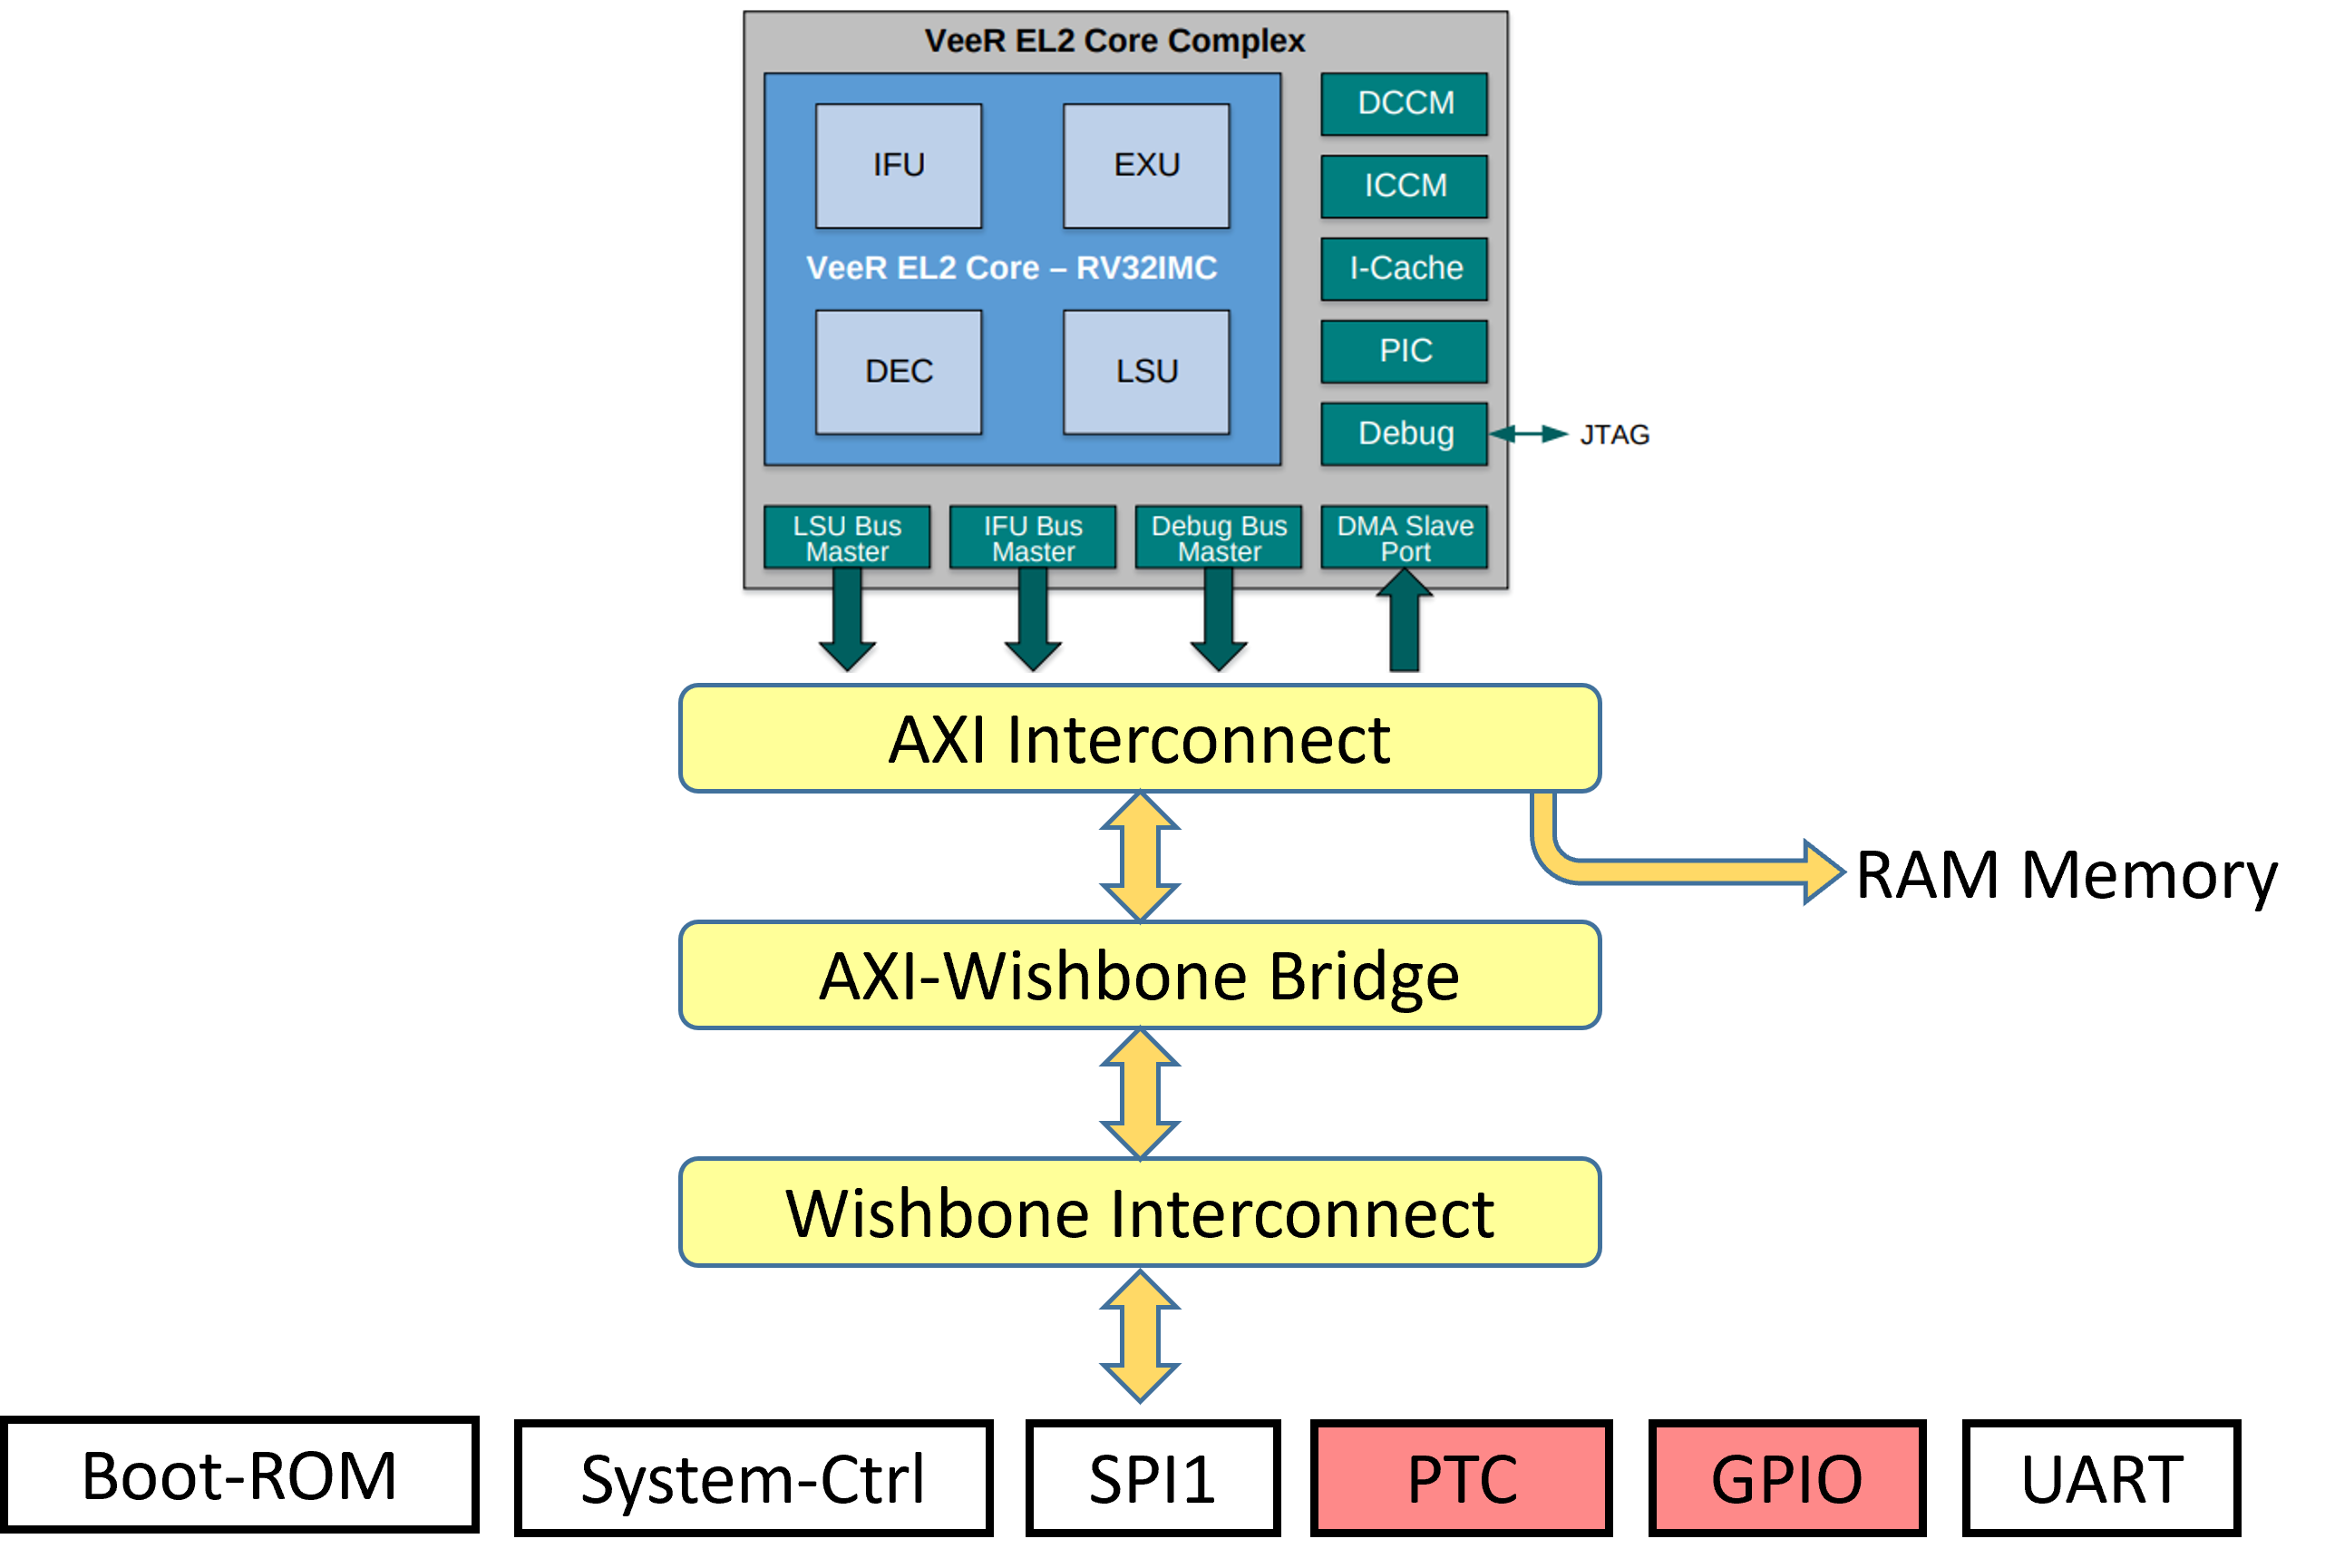
\includegraphics[width=\linewidth]{Images/VeeRwolf.png}
        \caption{VeeRwolf \ac{SoC} Integration Overview}
        \label{fig:el2_soc}
    \end{subfigure}
    \hfill
    \begin{subfigure}{0.35\textwidth}
        \centering
        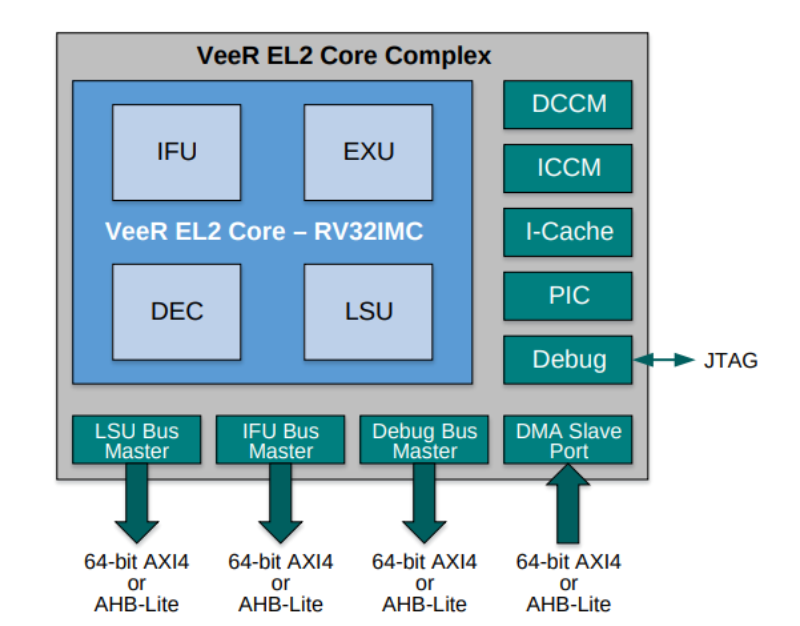
\includegraphics[width=\linewidth]{Images/VeeR EL2 Core.png}
        \caption{VeeR EL2 Core}
        \label{fig:el2_cpu}
    \end{subfigure}
    \caption{VeeRwolf EL2 Overview}
    \label{fig:el2}
\end{figure}

VeeR EL2 \cite{veer_el2} is a 32-bit, scalar, in-order, machine-mode-only \ac{CPU} with a four-stage pipeline. It implements RV32I with the compressed (C), multiplication and division (M), and a subset of bit-manipulation extensions. EL2 is delivered as a core complex with optional \ac{ICCM} and \ac{DCCM} memories, an optional instruction cache, three master ports for instruction fetch, load-store access, debug, and one slave \ac{DMA} port for external access to core memories. The external bus protocol can be configured as 64-bit \ac{AXI} or \ac{AHB}-Lite.

\begin{figure}[h]
\centering
    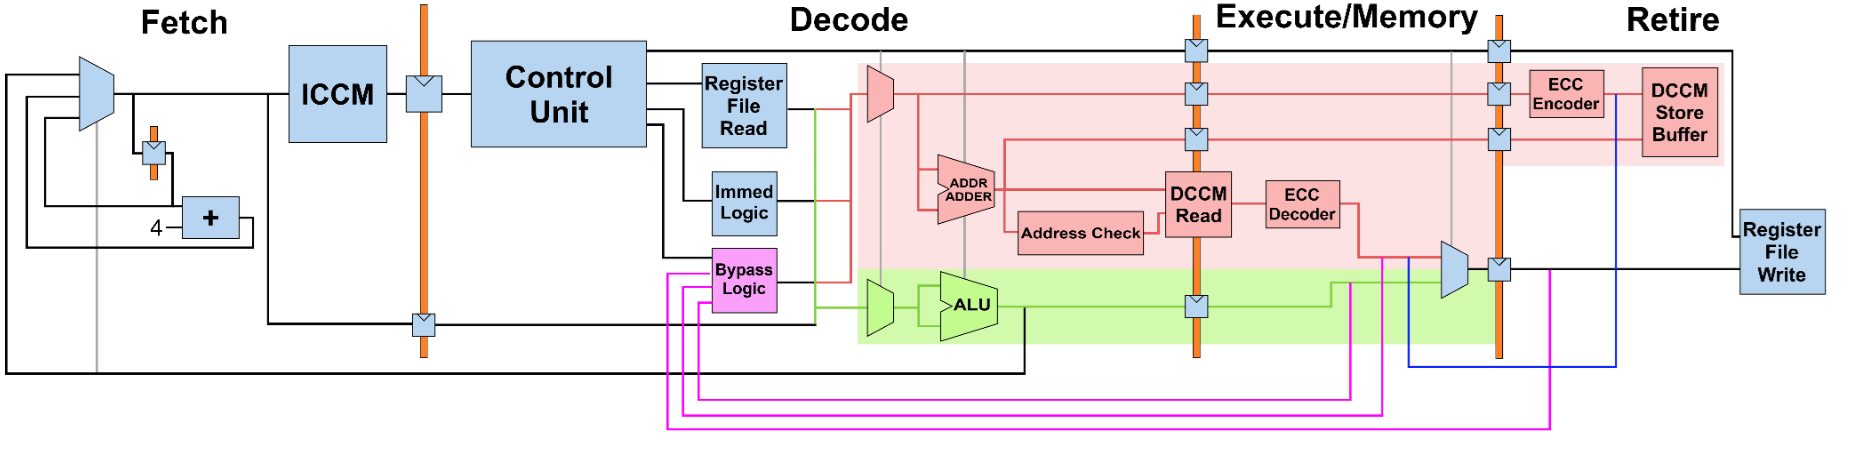
\includegraphics[width=0.85\textwidth]{./Images/EL2_Full_Pipeline.png}
    \caption{VeeR EL2's Full Pipeline}
    \label{fig:el2_pipeline}
\end{figure}

The pipeline, shown in \Cref{fig:el2_pipeline}, is organized into Fetch, Decode, Execute/Memory, and Retire stages. Fetch computes the next \ac{PC} and accesses the instruction source, either the instruction cache or \ac{ICCM}. Decode aligns/decodes instructions and selects operands. Execute/Memory performs arithmetic and control-flow operations and generates memory addresses. Retire completes memory and register writes. The implementation separates the arithmetic and control-flow path from the memory path, shown respectively as the I-pipe and LSU-pipe in the figure. In the studied configuration, \ac{DCCM} accesses include \ac{ECC} protection, stores use a write buffer, and bypass paths forward results from later stages back to Decode to reduce stalls.

VeeRwolf adds the \ac{SoC} blocks needed to execute software around the EL2 core complex. These include a boot ROM, system controller, \ac{UART}, \ac{SPI}, memory and peripheral interconnects, and an \ac{AXI}-to-Wishbone bridge. Since the available board at this stage was the Basys3 \cite{basys3}, the implementation followed the RVfpgaEL2-Basys3 flow, which uses the VeeRwolfX variant. This variant adds \ac{GPIO}, a \ac{PTC} timer, a controller for the four-digit seven-segment displays, \ac{AXI} RAM, \ac{JTAG} boundary-scan logic, and a clock generator.

The VeeRwolf EL2 study was mainly supported by the RVfpgaEL2-Basys3 course. This material provides guided labs for simulation and \ac{FPGA} execution, as well as debug software based on Catapult SDK, Catapult Studio, gcc-elf, gdb, and OpenOCD. Vivado is used when the \ac{SoC} must be rebuilt. The same environment also provides RVfpgaEL2-Trace for internal waveforms, RVfpgaEL2-Pipeline for pipeline visualization, RVfpgaEL2-ViDBo for virtual-board simulation, Whisper for instruction-set simulation, and PlatformIO projects for selected examples.



% #############################################################################
\section{VeeRwolf EL2 and Fault Tolerance}
\label{chap4:el2_design}

\begin{figure}[h]
\centering
    \includegraphics[width=0.9\textwidth]{./Images/EL2\_Full\_Pipe\_Faul\_Tolerance\_Baseline.png}
    \caption{Planned Implementations for VeeR EL2}
    \label{fig:el2_plan_impl}
\end{figure}

After studying the EL2 pipeline, three \ac{FTM} integration paths were planned and followed through, as shown in \Cref{fig:el2_plan_impl}. The first was register-level redundancy through \ac{TMR}, represented by the yellow registers, where each stored value would be replicated and voted before being used by the rest of the pipeline. The second was \ac{ECC} extension for storage structures, represented by the red blocks. Since \ac{ECC} already existed in the \ac{DCCM} path, the intended extension points were the register file and the \ac{ICCM}. The third was logic-level \ac{TMR} on the main address and control-flow adders, represented by the green blocks, targeting the \ac{PC} adder, the data-memory address adder, and the \ac{ALU} adder. 

When implementation began, the guided material and labs proved less useful for such low-level \ac{RTL} modification than anticipated. The planned mechanisms were harder to isolate than the diagram suggested, because EL2 contains long cross-module signal paths and tightly coupled control logic, so each modification required checking that pipeline behaviour, bypassing, memory access, and control dependencies were not being broken. To reduce this complexity before adding protection mechanisms, the design was first pruned into a simpler baseline. The branch predictor was removed, the multiplication and division paths were disabled, the bit-manipulation portion of the \ac{ALU} was removed, and both instruction and data caches were disabled so that instruction and data accesses relied on \ac{ICCM} and \ac{DCCM}. After this reduced baseline was operational, the planned implementations were attempted.

Pipeline-register \ac{TMR} was implemented by modifying the existing register wrapper to instantiate three register copies, vote their outputs with a newly developed voter, and propagate only the quorum value. \ac{TMR} was then applied to pipeline adders. The \ac{PC} adder and data-address adder were successfully triplicated because their interfaces were small and their signal boundaries were clear. The full \ac{ALU} \ac{TMR} was not completed because its integration reintroduced the same cross-module dependency problem and left unresolved implementation warnings. The final attempted extension was \ac{ECC} for additional memories beyond the already protected \ac{DCCM}. This was not completed. In EL2, close memory accesses still interact with the \ac{DMA} path, so extending memory protection required a deeper modification of the memory subsystem than the available time allowed. For this reason, the EL2-based implementation path was abandoned. The causes and consequences of this decision are discussed in \Cref{chap4:el2_lessons}.



% #############################################################################
\section{Lessons Learned and Conclusions}
\label{chap4:el2_lessons}

The VeeReolf EL2 conducted study and development, showed that the available RVfpgaEL2-Basys3 material was not enough for the low-level \ac{RTL} modifications required to develop \ac{Fatori-V}. The course was useful for understanding the system at a top level, executing examples, and using the available simulation and debug tools. However, it provided less support for restructuring \ac{RTL}, inserting new \acp{FTM}, and validating the design after deep modifications. Since the EL2 implementation contains tightly coupled control, memory, bypass, and \ac{SoC} interactions, each local \ac{FTM} change required broader verification across the pipeline and memory subsystem. This severely slowed the planned implementations.

As the intended scope of \ac{Fatori-V} became clearer, the project required more than adding protection logic to a core. It also required controlled \ac{FI}, metric collection, generated configuration files, benchmark automation, \ac{IP} generation, and Vivado-flow integration. Continuing with EL2 would therefore move too much effort into understanding and stabilizing the baseline instead of building the \ac{FTM} evaluation platform. For this reason, the EL2 path was abandoned, and the work moved to the second candidate discussed in \Cref{chap2:analysis}, lowRISC's Ibex, described next in \Cref{chap5:ibex}.
